\section{\bench{}: A Benchmark for Referential Ambiguity in Video}
\label{sec:benchmark}

\subsection{Dataset Construction}
\label{sec:construction}

\bench{} pairs 80 videos with 1{,}056 referentially ambiguous yes/no questions. Each question has an exhaustive list of $K$ readings. Each reading names its referent, restates the question with that referent resolved, and specifies a gold answer. Example: in Figure~\ref{fig:teaser}A the three readings refer to the first, second, and third attempts and restate the question. The gold answer is no for the first attempt and yes for the later two.

The videos feature similar co-occurring entities or recurring events, so short questions can underdetermine a referent. A vision-language model over-generates candidate questions with proposed reading lists. We keep only candidates that meet three requirements. First, the list must include the reading a viewer would reach first. Example: in a two-round game, \textit{``the winner''} in \textit{``does the winner celebrate?''} could mean the winner of either round or the overall winner. Viewers default to the overall winner. If a candidate lists only the two round winners, it omits this default reading and we discard it. Second, the mentioned referent must have a countable set of clearly visible groundings. Example: \textit{``the person''} in a street scene full of incidental passersby admits no stable exhaustive reading list, so it offers no fair target. Third, the ambiguity must arise from video entities and events rather than from a static layout. Example: in a split-screen broadcast showing two games side by side, \textit{``does the game end in a draw?''} is ambiguous only between the left and right halves of the frame, a static layout ambiguity that a single frame already exhibits. Human annotators validate every surviving question, checking that the reading list is exhaustive and that each gold answer holds (guidelines in Appendix~A). We release a public development split of 256 questions and withhold the 800-question test split.

Questions average 6.4 tokens, so ambiguity stems from video content rather than complex phrasing. The number of readings ranges from 2 to 56 with a mean of 6.1 (Figure~\ref{fig:stats}, left). Readings are consequential rather than interchangeable: in 92.0\% of questions at least two readings have different gold answers, so resolving to the wrong reading can change the user's answer.

\begin{figure}[t]
\centering
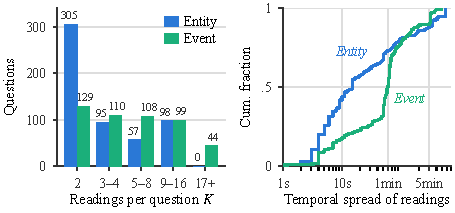
\includegraphics[width=\columnwidth]{figures/fig2_stats.pdf}
\caption{\bench{} statistics. \textbf{Left}: questions per number of readings $K$, by subset. \textbf{Right}: cumulative distribution of temporal spread, defined as the span between the earliest and latest gold evidence timestamps of a question's readings. For the event subset the median spread is one minute of footage. For a tenth of the questions it exceeds five minutes.}
\label{fig:stats}
\end{figure}

\paragraph{Large $K$.} We keep high-$K$ questions that image benchmarks exclude. RAcQUEt admits a question only when its target category has at most ten referents \citep{testoni2025racquet}. That design follows from scoring a single response, since cooperative speakers do not enumerate dozens of alternatives, so high-$K$ questions would be unfair there. Two properties make them fair here. First, they are combinatorial rather than vague: a high-$K$ case is a short question asked of footage where the same visible events recur many times. $K$ reaches 56 when a question relates two event types that recur eight and seven times, since each reading corresponds to one pair of occurrences. Validating such a list reduces to counting recurrences. Second, our protocol never requires enumeration: a clarifying question earns full credit at any $K$ (\S\ref{sec:protocol}). The scripted reply names a single intended reading, so the follow-up needs one answer, not 56. Large-$K$ questions therefore make clarification the natural strategy, which is the behavior the benchmark measures. We stratify all results by $K$ so no conclusion depends on the tail.

\paragraph{Subsets.} Following the two sources of ambiguity in Figure~\ref{fig:teaser}, \bench{} defines two subsets.\footnote{The remaining 11 questions mix both sources and are counted only in aggregate results.} In \textbf{\bench{}-Entity} (555 questions, 71 videos, mean $K$ of 4.6) several co-occurring entities match the mentioned attribute, as in Figure~\ref{fig:teaser}B, so readings are typically available within one scene and their gold evidence spans a median of 15 seconds. In \textbf{\bench{}-Event} (490 questions, 33 videos, mean $K$ of 7.9) the mentioned event or entity recurs, as in Figures~\ref{fig:teaser}A and \ref{fig:teaser}C, so readings are indexed by occurrence and separated in time with evidence that spans a median of one minute. In a tenth of questions, the earliest and latest evidence lie more than five minutes apart (Figure~\ref{fig:stats}, right). The two subsets operationalize the contrast from the introduction between readings that can be scanned within one scene and readings that must be recalled across episodes. Table~\ref{tab:comparison} situates the resource: among the benchmarks compared, \bench{} alone has readings separated in time and combines exhaustive reading lists, per-reading gold answers, and a scored clarification path.

\begin{table}[t]
\centering
\small
\setlength{\tabcolsep}{4.2pt}
\begin{tabular}{@{}lccccc@{}}
\toprule
Benchmark & Mod. & Time & Exh. & Gold & Inter. \\
\midrule
AmbigQA & text & \xmark & \cmark & \cmark & \xmark \\
Stengel-Eskin & image & \xmark & \cmark & \cmark & \xmark \\
RAcQUEt & image & \xmark & \xmark & \xmark & \xmark \\
ClearVQA & image & \xmark & \xmark & \xmark & \cmark \\
MUCAR & image & \xmark & \xmark & \xmark & \xmark \\
\midrule
\bench{} (ours) & video & \cmark & \cmark & \cmark & \cmark \\
\bottomrule
\end{tabular}
\caption{Comparison of \bench{} with ambiguity benchmarks in text \citep{min2020ambigqa}, visual QA \citep{stengeleskin2023chicken,testoni2025racquet,jian2025clearvqa}, and cross-modal resolution \citep{wang2025mucar}. \textbf{Time}: readings separated in time rather than co-present in one scene. \textbf{Exh.}: exhaustive human-validated reading lists. \textbf{Gold}: a gold answer per reading, so any response strategy is scorable. \textbf{Inter.}: a scored interactive clarification path.}
\label{tab:comparison}
\end{table}


\subsection{Interactive Protocol and Metrics}
\label{sec:protocol}

\begin{figure*}[t]
\centering
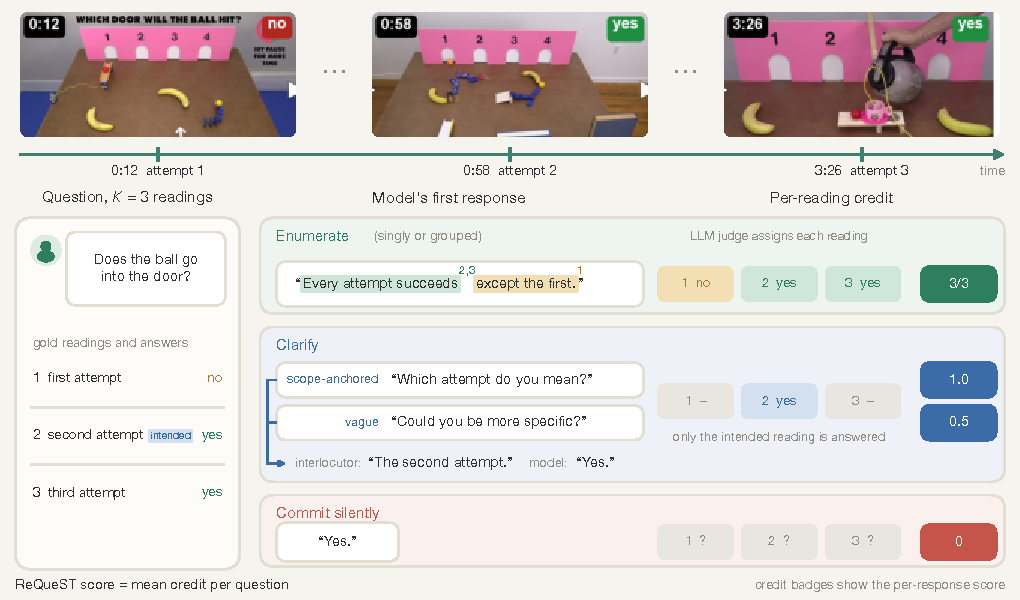
\includegraphics[width=0.90\textwidth]{figures/fig_overview.pdf}
\caption{Protocol and scoring of \bench{}. A model receives a video and a question whose $K$ readings and gold answers are annotated in advance (left). Its first response takes one of three routes (rows). For an enumeration, the judge assigns each reading the answer the response determinately entails: the highlighted spans of the grouped reply match the reading cells they cover, so credit is proportional. A scope-anchored clarification earns full credit and a vague one half credit, after the interlocutor names the intended reading. A silent commitment identifies no reading and earns nothing. The \textbf{\bench{} score} is the mean credit across questions.}
\label{fig:overview}
\end{figure*}

\paragraph{Protocol.} Figure~\ref{fig:overview} summarizes the interaction. A model receives the video and the question with a prompt that permits three behaviors: answer directly, answer for every reading, or ask a clarifying question. A validated classifier (\S\ref{sec:judge}) assigns the first response to one of five types: \textit{enumeration}, \textit{scope-anchored clarification} (names the ambiguous phrase, \textit{``which man do you mean?''}), \textit{vague clarification} (asks for more information without locating the ambiguity), \textit{single commitment}, or \textit{refusal}. For each question, we designate one reading as the intended reading via a deterministic hash of the question ID. The draw spreads intents uniformly over readings and stays identical for every model and run. A scripted interlocutor with a \textit{fixed intention} answers every clarification by naming the intended reading verbatim from its gold description, regardless of how the model phrases its request. The model must then answer for the named reading. The dialogue ends after at most three model turns. Letting the interlocutor adopt a reading the model proposes would let models steer toward easier readings, which would make scores incomparable across models.

\paragraph{Scoring.}
We report the \textbf{\bench{} score} as the mean per-question credit. Each question contributes one credit from whichever route the model takes, so we pool enumeration and clarification. For an intended reading drawn uniformly from the list, the score estimates the probability that the response determinately answers it correctly. We assign credit as follows:
\begin{itemize}
\item \textbf{Enumerations} earn credit proportional to the fraction of the $K$ readings answered correctly. The judge credits what the response determinately entails, whether stated singly or in groups. For example, the grouped reply in Figure~\ref{fig:overview}, \textit{``Every attempt succeeds except the first.''}, determinately answers all three readings. Hedged or vague coverage earns no credit, for instance \textit{``probably every attempt succeeds''} or \textit{``the attempts succeed''}.
\item \textbf{Clarifications} earn full credit at any $K$ if scope-anchored. Vague clarifications earn half credit for identifying ambiguity while forcing the user to locate the specific source of confusion. Both require a correct follow-up answer. We score the follow-up against the gold answer of the intended reading, exactly one comparison rather than $K$ comparisons.
\item \textbf{Commitments} and refusals earn zero credit. Even a correct commitment provides no signal for the user to identify which reading the model answers.
\end{itemize}
Answering all $K$ readings correctly satisfies the \textbf{strict-$K$} criterion, which we report as a diagnostic. We decompose enumeration credit into \textit{reading coverage}, the fraction of gold readings a response addresses, and \textit{conditional correctness}, the accuracy on the readings it addresses. Their gap separates failures to find readings from failures to answer them, the distinction at the center of this paper.

\paragraph{Silent misinformation.} Commitments vary in harm, so we quantify it directly. A dedicated mapping step (\S\ref{sec:judge}) assigns each committed response to the gold reading it answers. The \textbf{silent misinformation rate (SMR)} is the fraction of questions where the model commits to a reading other than the intended one and gives an answer that differs from the intended reading's gold answer. The user then receives a confident answer that is wrong for their intended reading with no signal that anything went wrong. When the delivered answer matches the intended reading's gold answer, we count \textit{misgrounding}, a correct answer reached through the wrong reading, and report it separately.

\paragraph{Reproducibility.} We fix interlocutor replies, gold answers, and intents before evaluation, so every model faces the same dialogue. We evaluate each model once with frozen weights, so it cannot learn a strategy against the fixed reply (details and worked dialogues in Appendix~C).

\subsection{Judge and Validation Suite}
\label{sec:judge}


An automatic suite with three components computes the metrics above: a five-way response-type classifier, an answer-correctness judge that assigns each gold reading the answer the response determinately entails whether stated singly or in groups, and a reading-selection mapping that assigns a committed response to the reading it answers. The mapping matters because SMR and the selection analysis of \S4 both depend on it. It is a classifier in its own right, so we validate it rather than treat it as preprocessing.

Table~\ref{tab:validation} summarizes validation. The judge is a fixed Gemini-3-Flash configuration at temperature 0. We characterize re-run stability, cross-family agreement, and human agreement. Re-running the same judge reproduces response-type labels almost exactly ($\kappa \geq 0.98$) and per-reading assignments at 99.1\% agreement (Pearson $r = 0.98$). A GPT-4o judge agrees on 96.2\% of per-reading assignments ($r = 0.96$) and is the sole source of the lower enumeration $\kappa$, with disagreement concentrated in grouped statements at the margin. The model differences in \S4 are substantially larger than these judge disagreements. A single annotation session provides the human column: agreement with human annotators for all five components, inter-annotator agreement on reading-list exhaustiveness, and a 30-example adjudicated error audit (Appendix~B).
